\section{Definição}

\begin{frame}[fragile]{UFDS}

    \metroset{block=fill}
    \begin{block}{Definição}
        \textit{Union-find disjoint set} (UFDS) é uma estrutura de dados que mantém uma coleção
        de conjuntos $\lbrace S_1, S_2, \ldots, S_N\rbrace$ disjuntos, isto é, $S_i\cap S_j =
        \emptyset$ se $i\neq j$. Há duas operações básicas, com complexidade $O(\log N)$: a 
        \textbf{união} (\texttt{union\_set(A, B)}) de dois conjuntos disjuntos e a identificação 
        do \textbf{representante} da união de conjuntos que o conjunto \texttt{S} pertence 
        (\texttt{find\_set(S)}).
    \end{block}

\end{frame}

\begin{frame}[fragile]{Características da UFDS}

    \begin{itemize}
        \item A UFDS foi proposta em 1971 por J. D. Hopcroft e J. D. Ullman

        \item Ela é composta por uma floresta de árvores

        \item Cada árvore representa uma união de subconjuntos

        \item A raiz de cada árvore é o representante da união

        \item Cada nó da árvore representa um dos conjuntos que compõem a união

        \item Conjuntos representados por árvores distintas são disjuntos

        \item Duas árvores podem ser unidas tornando a raiz de uma delas filha da raiz da outra

        \item Se a árvore com o menor número de elementos for incorporada na de maior número de
            elementos, a união terá complexidade $O(\log N)$
    \end{itemize}

\end{frame}

\begin{frame}[fragile]{Visualização de uma UFDS}

    \begin{figure}
        \centering

        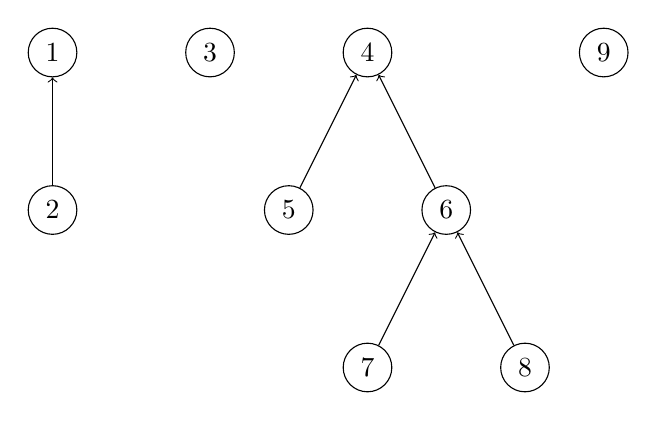
\begin{tikzpicture}
            \node[draw, circle] (A) at (0, 4) { 1 };
            \node[draw, circle] (B) at (0, 2) { 2 };

            \node[draw, circle] (C) at (2, 4) { 3 };

            \node[draw, circle] (D) at (4, 4) { 4 };
            \node[draw, circle] (E) at (3, 2) { 5 };
            \node[draw, circle] (F) at (5, 2) { 6 };
            \node[draw, circle] (G) at (4, 0) { 7 };
            \node[draw, circle] (H) at (6, 0) { 8 };

            \node[draw, circle] (I) at (7, 4) { 9 };

            \draw[->] (B) edge (A);
            \draw[->] (E) edge (D);
            \draw[->] (F) edge (D);
            \draw[->] (G) edge (F);
            \draw[->] (H) edge (F);

        \end{tikzpicture}
    \end{figure}

\end{frame}
